\pagestyle{fancy}
%%%%%%%%%%%%%%%%% ML
Machine learning (ML) is a branch of \textbf{artificial intelligence (AI)} and computer science which focuses on the use of data and algorithms to imitate the way that humans learn, gradually improving its accuracy. 
The learning part is called training and is performed on training data, the trained algorithm is then tested on test data. 
Through the use of statistical methods, algorithms are trained to make classifications or predictions \cite{ibm}. The term "Machine Learning" was first introduced in a paper from 1959, where the computer was trained to play the game of checkers \cite{ml0}. ML can be divided into three primary categories based on how they learn \cite{ibm}:
\begin{itemize}\thispagestyle{fancy}
    \item \textbf{supervised learning} - using labeled datasets to train algorithms that classify data or predict outcomes accurately. As input data is fed into the model, it adjusts its weights until the model has been fitted appropriately
    \item \textbf{unsupervised learning} - using machine learning algorithms to analyze and cluster unlabeled datasets. These algorithms discover hidden patterns or data groupings without the need for human intervention
    \item \textbf{reinforcement machine learning} -  behavioral machine learning model that is similar to supervised learning, but the algorithm is not trained using sample data. This model learns using the trial and error method
    \end{itemize}
The most known uses of ML are i.e. speech recognition, computer vision, recommendation engines. Furthermore, it has been also successfully used already in the high-energy physics (more specifically the subcategory of ML, the \emph{deep learning}, which automates much of the feature extraction piece of the process, requiring less human intervention to learn), for tasks as simulating the calorimeter response in the LHCb experiment \cite{lhcb}, and inspection of the silicon micro-strips of the STS detector in the CBM experiment \cite{zenia} (shown on Figure \ref{zenia ml}).
\begin{figure}[H]
    \centering
    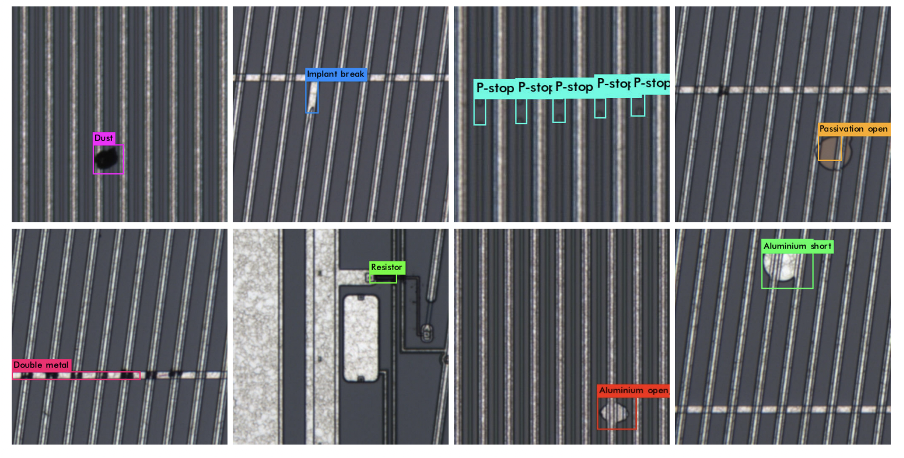
\includegraphics[width=.65\textwidth]{inz_szablon_new/img/ml-sts.png}
    \caption{Various surface defects on the silicon sensor identified using deep neural network \cite{zenia}}
    \label{zenia ml}
\end{figure}


%%%%%%%%%%%%%%%%%%%%%%%%%%%% XGBoost
\section{XGBoost}
XGBoost  is a \textbf{decision-tree-based, supervised} ML algorithm that uses gradient boosting, available as an open-source package. 
It has unique tree structure and it offers parallel processing and regularization parameters. \cite{xgboost}. It is highly efficient when used with e.g., tabular data. \cite{shahid} It combines three elements (also shown on Figure \ref{xgboost diagram}): 
\begin{itemize}
    \item \textbf{Decision trees} - Graphical representation of possible decisions based on certain conditions
    \item \textbf{Random Forest} - Selecting a random subset of features from multiple decision trees and \emph{bagging} - making a decision based on the majority of their predictions
    \item \textbf{Gradient Boosting} - Applying gradient descent algorithm to minimize the errors from random forests to train the algorithm \cite{xgboost1}\\
\end{itemize}


Contrary to normal decision trees, it returns the \textbf{probability} of a certain decision (not a 0-1 decision) and trains itself given the error of its predictions (using mentioned before \emph{gradient boosting}).
\begin{figure}[H]
    \centering
    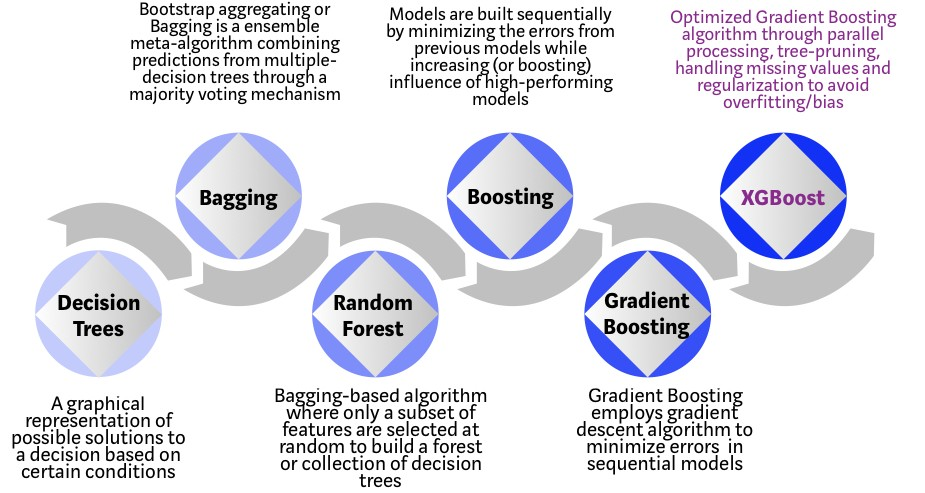
\includegraphics[width=.86\textwidth]{inz_szablon_new/img/xgboost_diagram.jpeg}
    \caption{Evolution of XGBoost Algorithm from Decision Trees \cite{xgboost1}}
    \label{xgboost diagram}
\end{figure}
Each XGBoost model (and in general almost all ML models) has \textbf{hyperparameters} - parameters that describe the model itself (and have a big impact on its results). The most important ones, which will be changed in this work are (in xgboost version: 1.3.3) \cite{xgboost-doc}:
\begin{itemize}
    \item \textbf{max\_depth} (default value = 6) - Maximum depth of a tree. Increasing this value will make the model more complex and more likely to overfit
    \item \textbf{gamma} (default = 0) - Minimum loss reduction required to make a further partition on a leaf node of the tree. The larger gamma is, the more conservative the algorithm will be
    \item \textbf{alpha} ( default = 0) - A L1 regularization term on weights. Increasing this value will make the model more conservative
    \item \textbf{learning\_rate} (default = 0.3) - Step size shrinkage used in update to prevent overfitting. After each boosting step, we can directly get the weights of new features, and eta shrinks the feature weights to make the boosting process more conservative
    \item \textbf{n\_estimators} (default = 6) - Number of gradient boosted trees. Equivalent to number of boosting rounds\\
\end{itemize}

There are multiple ways to choose the optimal configuration (values) of hyperparameters, notably Grid Search, Random Search,  and Bayesian Optimisation \cite{compare hyper}. The comparison between them is shown in  Table \ref{hyperparams} (the +/- sign means that time needed is shorter than in Grid Search, but longer than in Bayesian Optimisation). Following the comparison and the method chosen earlier by the CBM-ML group \cite{shahid}, \textbf{Bayesian Optimisation} will be used in this work.\\

\begin{table}[h]
\begin{tabular}{|l|l|l|l|}
\hline
\textbf{} &
  \textbf{Grid Search} &
  \textbf{Random Search} &
  \textbf{Bayesian Optimisation} \\ \hline
Checks every configuration & + & - & - \\ \hline
\begin{tabular}[c]{@{}l@{}}Not much time needed to find the\\  optimal configuration\end{tabular} &
  - &
  +/- &
  + \\ \hline
Learns with each step      & - & - & + \\ \hline
\end{tabular}
\caption{Comparison of hyperparameters optimization methods}\label{hyperparams}
\end{table}

%%%%%%%%%%%%%%%Comparsion optimisatiopn